\documentclass[10pt,a4paper]{article}
\usepackage[letterpaper,margin=0.75in]{geometry}
\usepackage[utf8]{inputenc}
\usepackage{mdwlist}
\usepackage[T1]{fontenc}
\usepackage{textcomp}
\usepackage{tgpagella}
\pagestyle{empty}
\setlength{\tabcolsep}{0em}

\usepackage[defaultfam,tabular,lining]{montserrat} %% Option 'defaultfam'
%% only if the base font of the document is to be sans serif
\usepackage[T1]{fontenc}
\renewcommand*\oldstylenums[1]{{\fontfamily{Montserrat-TOsF}\selectfont #1}}


\usepackage{graphicx}

\begin{document}
\vspace*{\fill}
\begin{center}
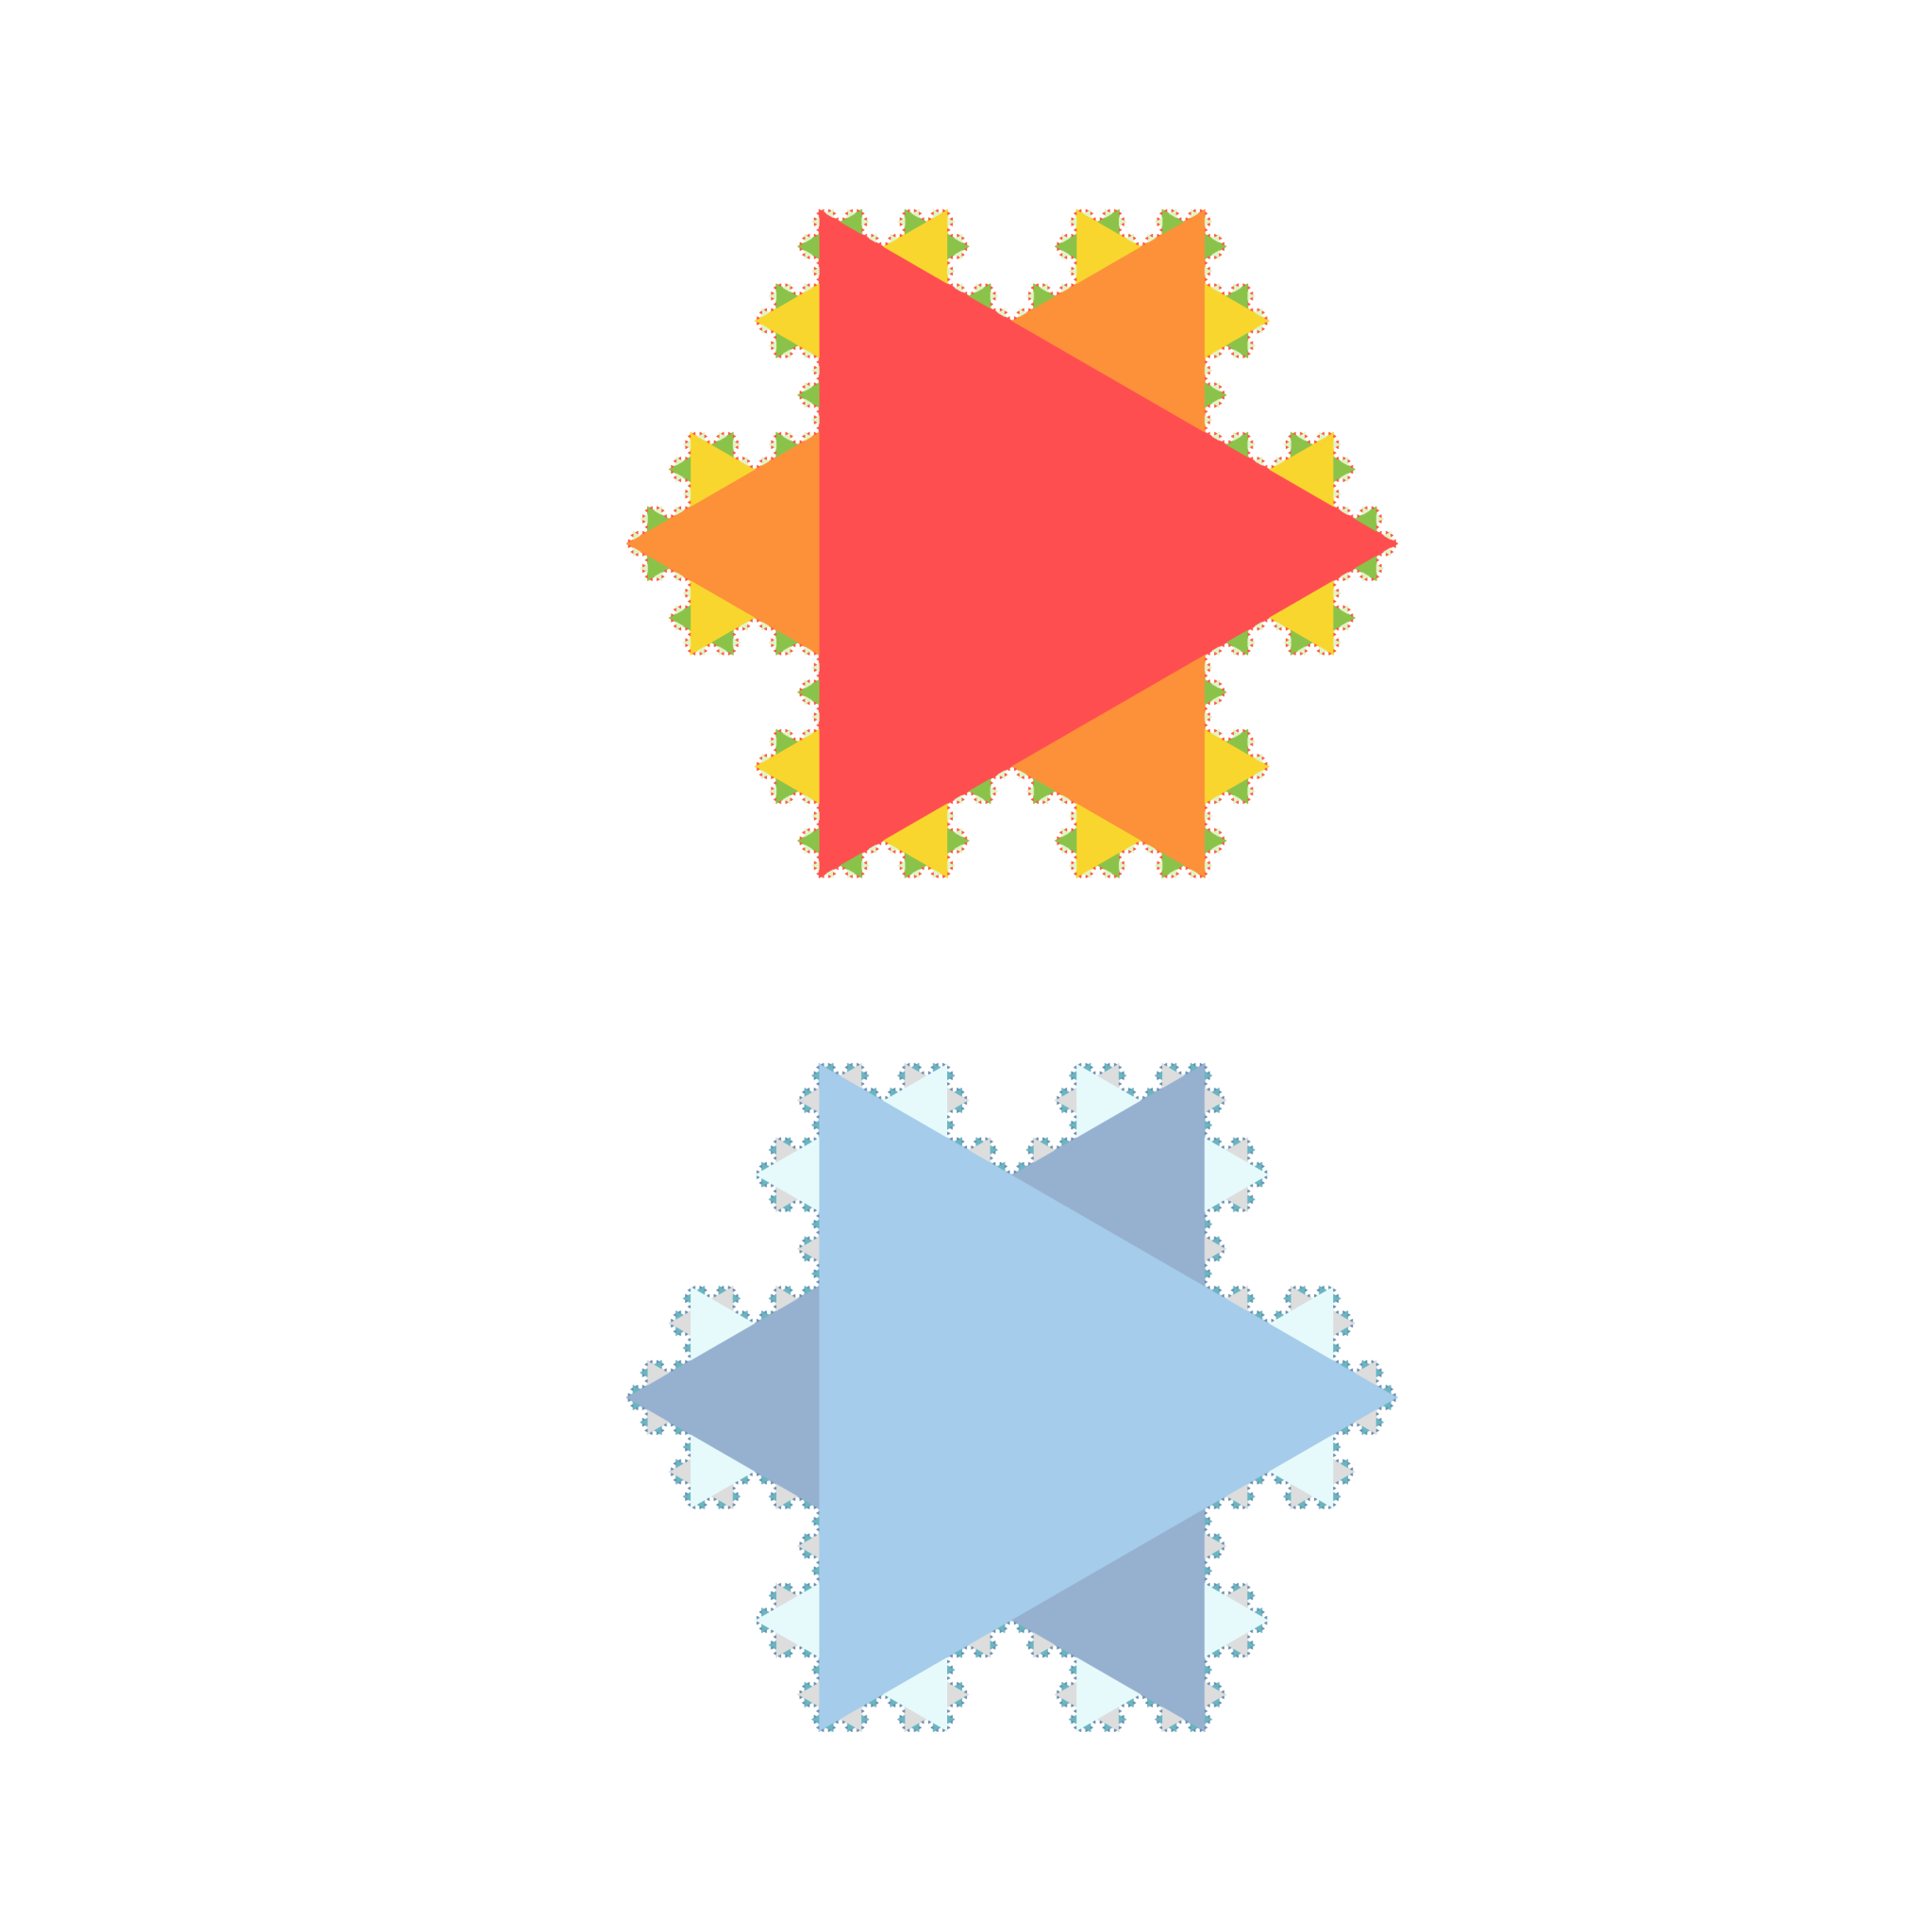
\includegraphics[width=\textwidth]{../Images/summer_winter.png}
\end{center}
\vspace*{\fill}

\begin{center}
\tiny
The snowflake fracture is a shape with infinite perimeter but finite area. It is made by adding smaller and smaller triangles to the existing shape. It was first defined in 1904 by the Swedish mathematical Helge von Koch.
\end{center}

\end{document}